\documentclass[fleqn]{article}
\usepackage[utf8]{inputenc}
\usepackage[margin=1in]{geometry}
\usepackage{mathtools}
\usepackage{graphicx}
\usepackage{listings}
\usepackage[section]{placeins}
\usepackage{pdfpages}

\graphicspath{ {images/} }

\begin{document}
\title{MiniPL Interpreter}
\author{Tuomas Tirronen}
\date{\today}
% \level{CSM14204 Compilers}
\maketitle
\newpage

\tableofcontents

\newpage

\section{Solution architecture}

The interpreter is divided in to components as described in figure 1.
\par
Scanner reads the source code one character at a time, constructing valid tokens and passing them to the parser.
\par
The parser matches the input token stream against the syntactic rules of the context-free grammar, and constructs an abstact syntax tree during the process.
This solution does not build a parse tree, but instead it directly creates the abstract syntax tree.
\par
The scanning and parsing process is performed in one pass: The parser requests new tokens from the scanner, which then processes the source code and returns the next token.
When the parser is finished, the abstact syntax tree is retrurned to the main program.
\par
Semantic analyzer analyzes the semantic correctness of the abstact syntax tree, e.g. allowed operations, type checking and performs the variable declaration (creates an entry in the symbol table).
Semantic analyzer implements the visitor pattern to traverse the abstract syntax tree.
\par
Interpreter also implements the visitor pattern and it interprets each node in the abstact syntax tree.
The interpretation is relatively simple, as the evaluation and symbol lookups are done in the Evaluator component.
\par
The evaluator is responsible for evaluating the different expressions in the source program. Evaluator also implements the visitor pattern.


{\centering
    \vspace*{1cm} 
    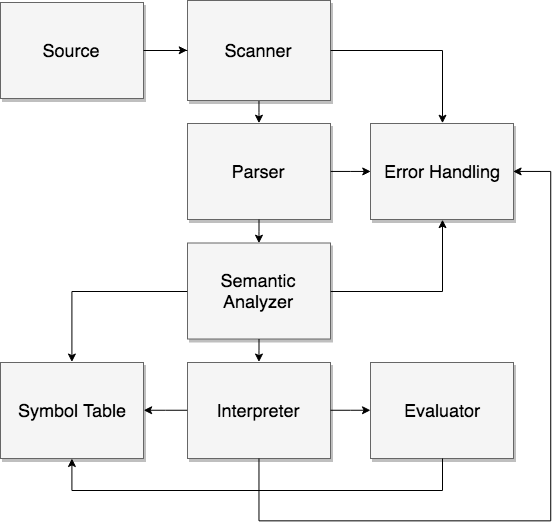
\includegraphics[width=0.5\textwidth]{architecture}
    \\Figure 1: Overall architecture of the interpreter.
    \par
}
 
\newpage
\section{Token patterns}

\begin{gather*}
    integer \Rightarrow digit \ digit* \\
    boolean \Rightarrow 0 \ | \ 1 \\
    string \Rightarrow letter \ letter* \\    
    identifier \Rightarrow letter \ (letter \ | \ digit)* \\
    letter \Rightarrow  A \ | \ B \ | \ . . . \ | \ Z \ | \ a \ | \ b \ | \ . . . \ | \ z \\
    digit \Rightarrow  0 \ | \ 1 \ | \ 2 \ | \ . . . \ | \ 9
\end{gather*}

\section{Context-free grammar}
\begin{gather*}
    program \Rightarrow block \\
    block \Rightarrow statement \ (statement)* \\
    statement \\
    \quad \Rightarrow "var" \ identifier \ ":" \ type \ [ ":=" expression ] \\
    \quad \Rightarrow identifier \ ":=" \ expression \\
    \quad \Rightarrow "for" \ identifier \ "in"  expression \ ".." \ "do" \ block \ "end" \ "for" \\
    \quad \Rightarrow "read" \ identifier \\
    \quad \Rightarrow "print" \ expression \\
    \quad \Rightarrow "assert" \ "(" expression ")" \\
    expression \Rightarrow term \ (("+" \ | \ "-") \ term)* \\
    term \Rightarrow factor \ (("*" \ | "/" | "<" | "\&" | "=") \ factor)*  \\
    factor \Rightarrow integer \ | \ string \ | \ boolean \ | \ identifier \ | "(" \ expression \ ")" \ | \ "!" factor
\end{gather*}

\newpage
\section{Abstract syntax trees}
The abstract syntax tree is composed of different types of nodes, all inherited from an abstact node class.
\par
Node types \textit{BinOpNode}, \textit{UnOpNode}, \textit{IntNode},\textit{StrNode}, \textit{BoolNode} and \textit{IdNode}
are constructed with the token information. The information of the \textit{value} attribute varies between node types.
For operation nodes (\textit{BinOpNode} and \textit{UnOpNode}), it stores the operation symbol (\textit{+}, \textit{-}, \textit{*} or \textit{/}).
For \textit{IdNode}, it stores the label of the symbol, and for literal nodes (\textit{IntNode}, \textit{StrNode}, \textit{BoolNode}),
it stores the value of the terminal as a string.
\par
A node also stores information on its location in the source code. This is done by saving the row and column numbers that are obtained during the scanning process.

{\centering
    \vspace*{1cm} 
    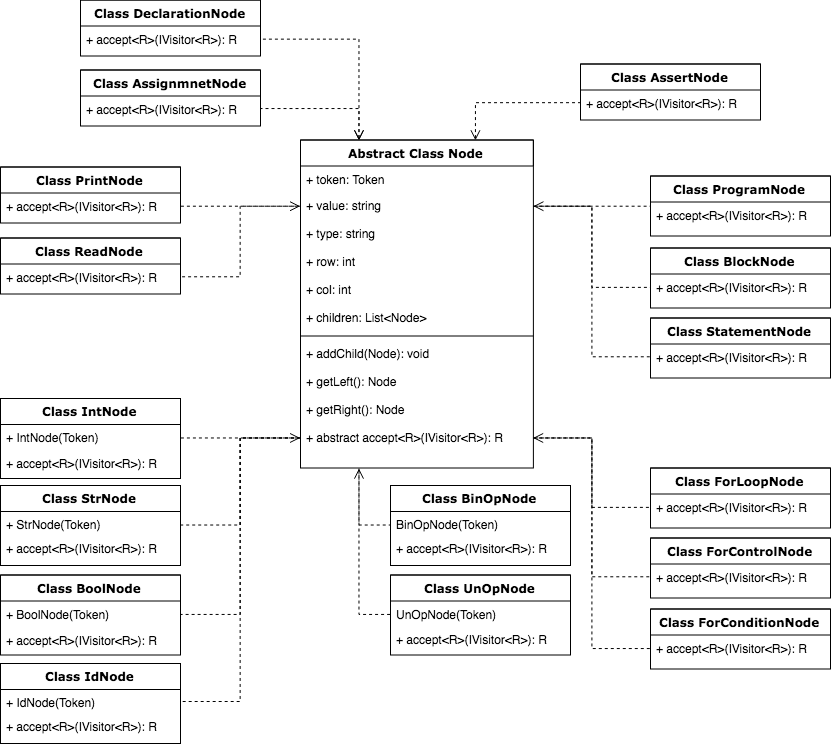
\includegraphics[width=0.8\textwidth]{ast}
    \\Figure 2: Class diagram of the abstact syntax tree.\par
}

\newpage
The abstact syntax tree is constructed during the parsing process. As an example, for the following source program, an abstact syntax tree is build as shown in Figure 3.

\begin{lstlisting}
    var X : int := 4 + (6 * 2);
    print X;
\end{lstlisting} 
 
{\centering
    \vspace*{1cm} 
    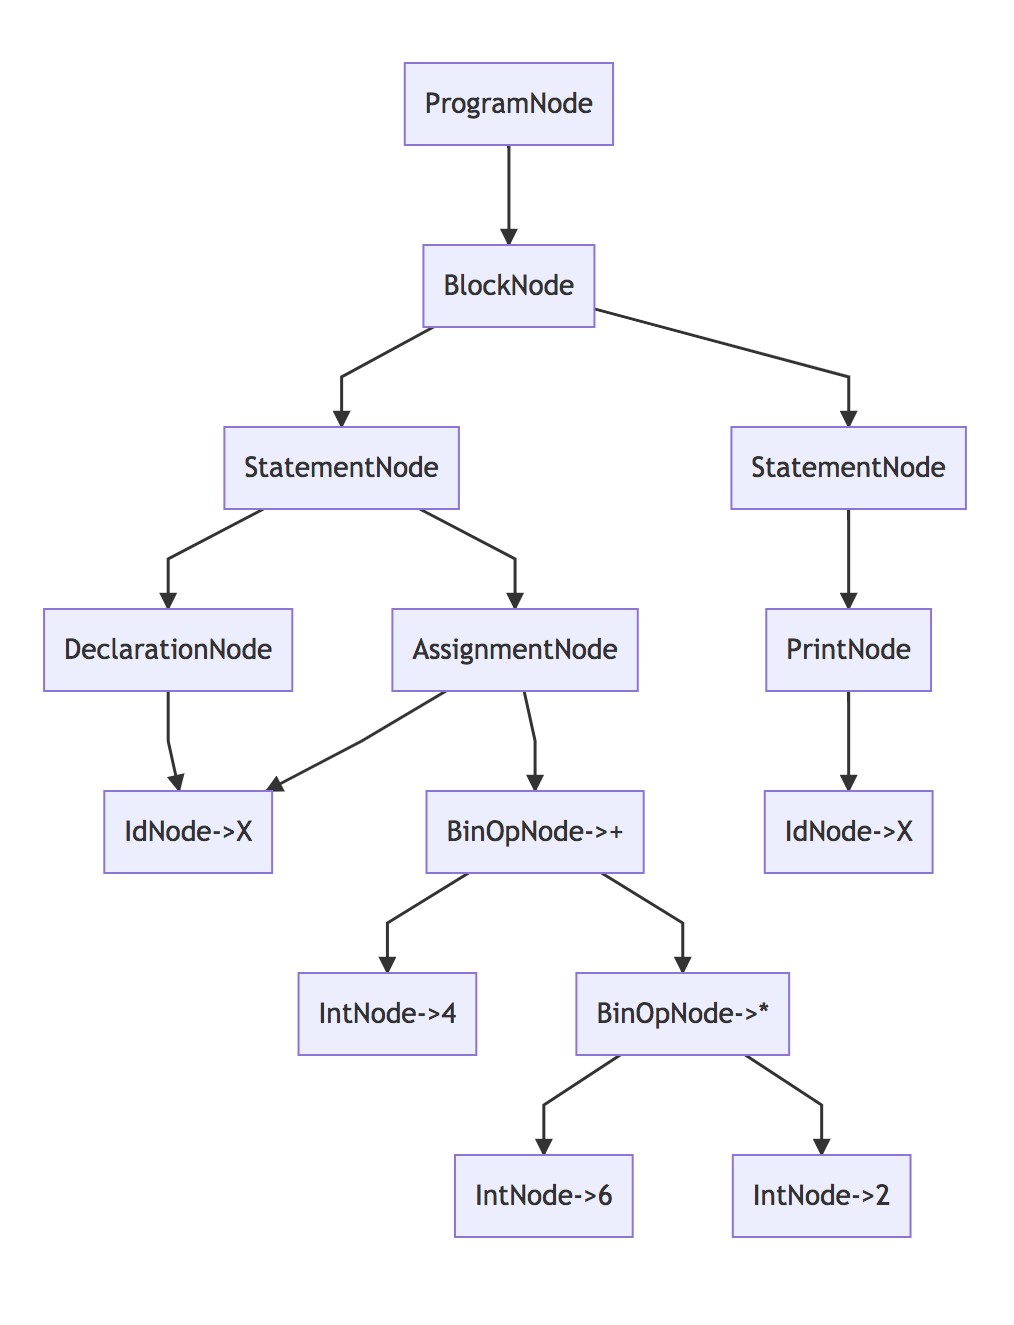
\includegraphics[width=0.7\textwidth]{sample1}
    \\Figure 3: Example of an AST instance.\par
}


\newpage
\section{Error handling}
Error handling component is used by scanner (lexical errors), parser (syntax errors), semantic analyzer (semantic errors) and interpreter (runtime errors).
The aim for each component is to save the errors in a global error table, try to recover from it and continue their process;
Scanner by returning a special unknown token and parser by starting again from the next statement (a token followed by \textit{;}).
\par
If the source program is found free from lexical and syntax errors, the program continue with the semantic analysis to ensure correct data types in operations and symbol usage.
Once there are no semantic errors after the analysis, the source program will be interpreted.
The interpreter will then detect runtime errors, that can be derived from user interaction, namely from providing invalid input for the \textit{read} operation.
\par
The evaluator assumes all the possible errors are found during previous components in the pipeline, so it does not make use of the error component.
\section{Testing}
\section{Limitations}
\par
The known limitations and bugs for the interpreter are the following:

\begin{itemize}
    \item Comment at the end of the source program will cause the scanner to break.
    \item The symbol table is not scoped
    \item Testing is not comprehensive
    \item Code is not properly commented
\end{itemize}

\section{Usage}
The interpreter requires to have Microsoft .NET environment installed. To interpret a MiniPL program, navigate to the \textit{src} directory and run the following command:
\newline
\newline
\texttt{
    dotnet run \textit{your\_program}
}

\appendix
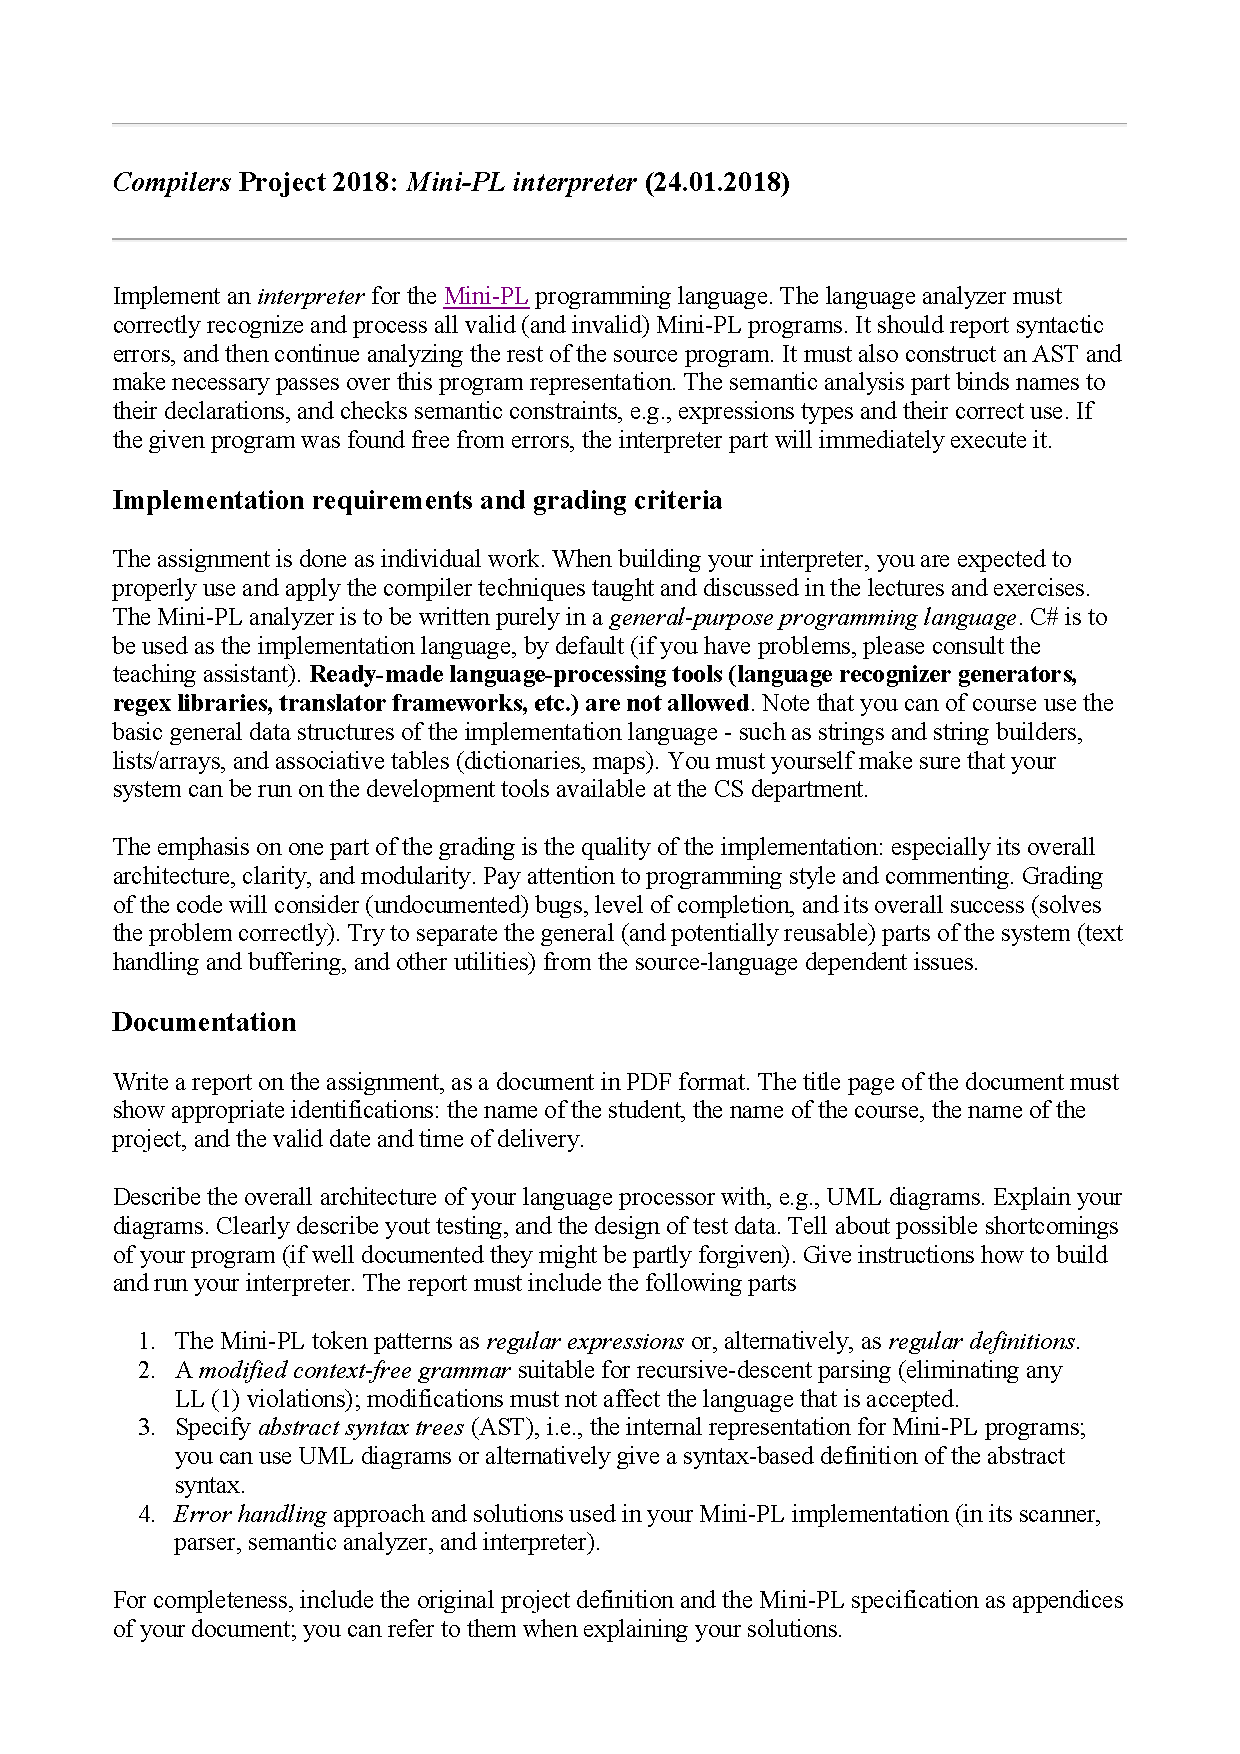
\includepdf{appendix/assignment.pdf}
\appendix
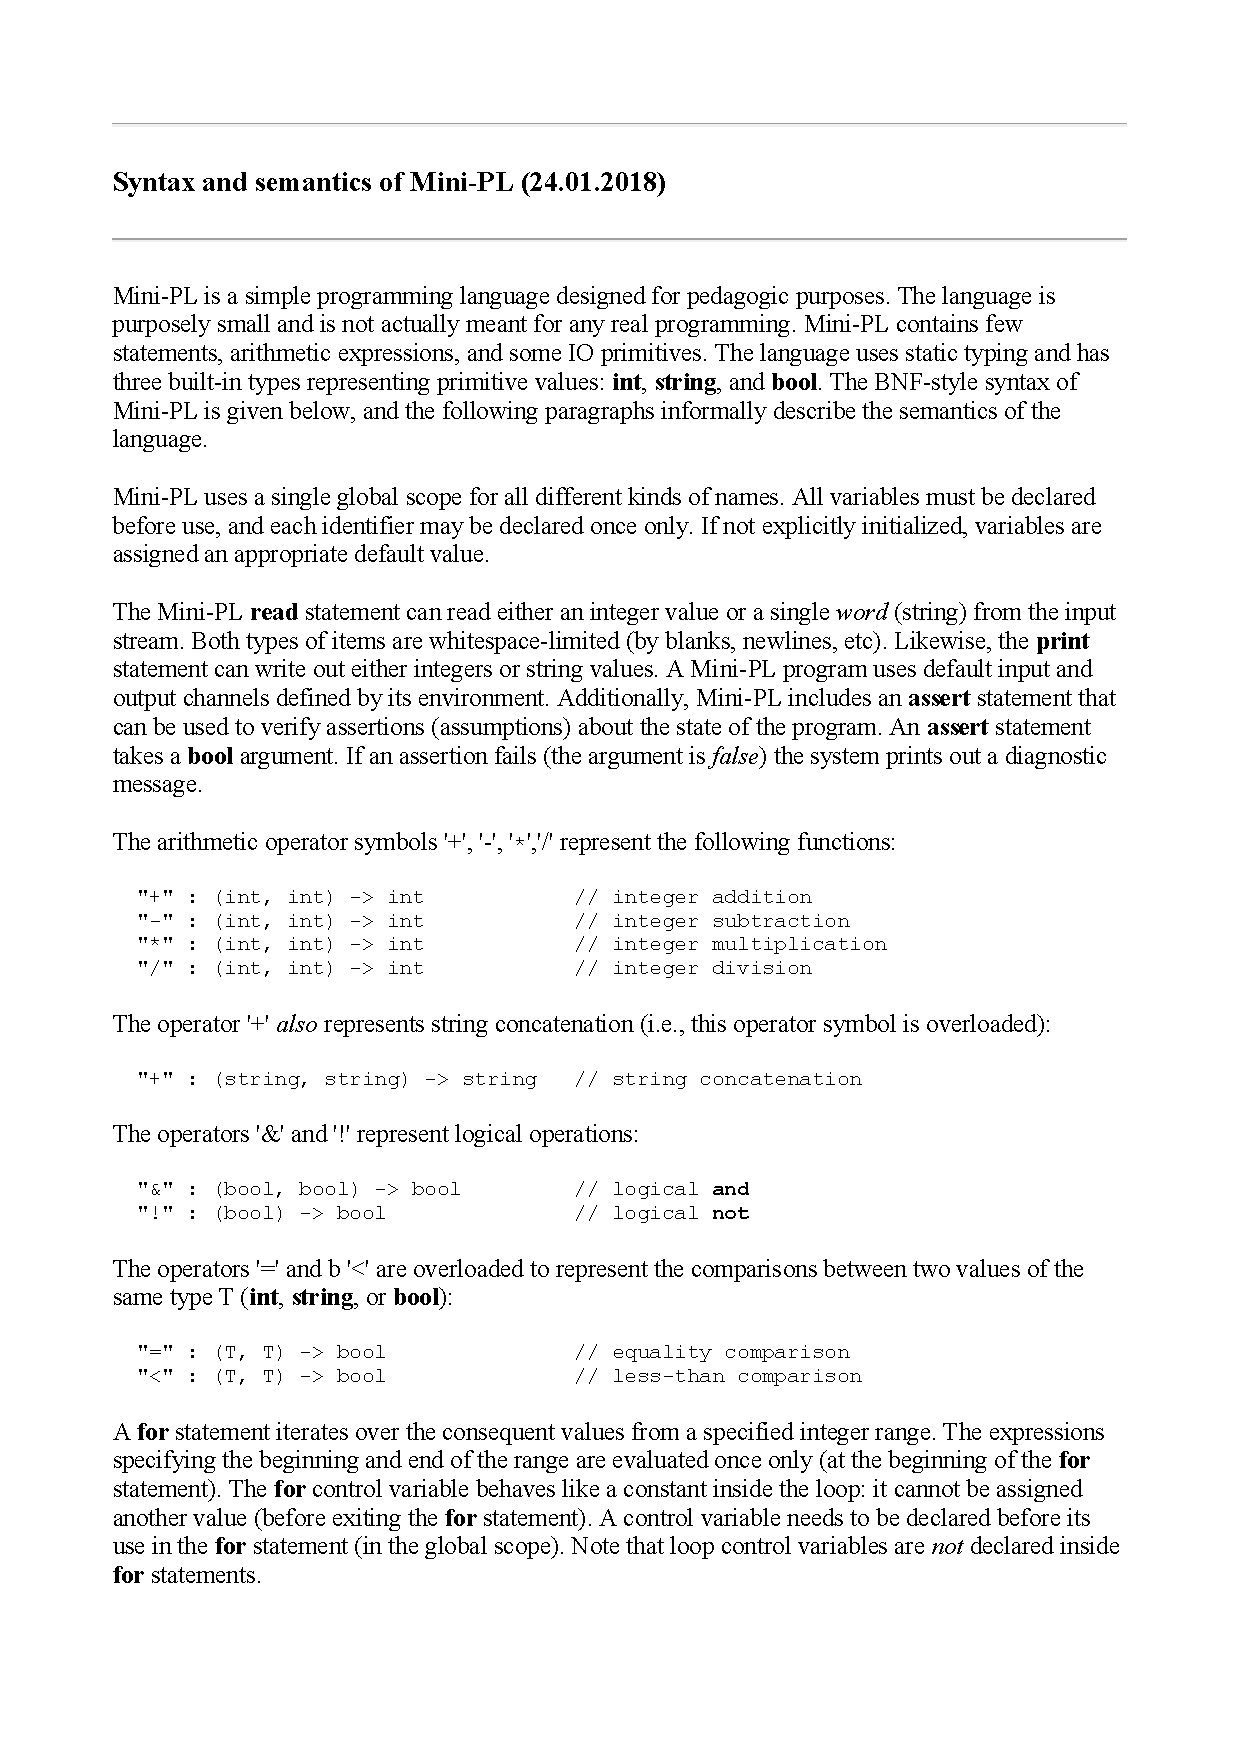
\includepdf{appendix/syntax.pdf}
\end{document}